\begin{pastexam}[label={px:ntu-110-ie-ds-19}]{臺大工工所 110 學年度 第 19 題}
（複選；每題 5 分，每答錯一個選項倒扣 1 分至該題 0 分止）

Consider the splay tree in Figure 1. Which of the following statements are true?\\
(Assume bottom-up splay, also assume the Join() operation splays on the maximum element in the left
tree, which then attaches the right tree.)
\begin{enumerate}[label=(\Alph*)]
\item In Figure 1, after deleting key 26, then key 33 is a child of key 48.
\item In Figure 1, after deleting key 26, then key 17 is the root.
\item In Figure 1, after inserting key 75, then key 64 is an ancestor of key 99.
\item In Figure 1, after inserting key 75, then key 33 is a descendant of key 55.
\item In Figure 1, after inserting key 75, then key 75 is the root.
\end{enumerate}
\begin{center}
\begin{tikzpicture}[v/.style={circle,draw,thick,inner sep=1pt,minimum size=6mm,font=\small\sffamily},>={Stealth[length=2mm]}]
\node[v] (55) at (0,0) {55};
\node[v] (48) at (-0.9,-0.95) {48}; \node[v] (64) at (0.8,-0.95) {64};
\node[v] (33) at (-1.8,-1.9) {33}; \node[v] (82) at (1.7,-1.9) {82};
\node[v] (26) at (-2.7,-2.85) {26}; \node[v] (71) at (1.1,-2.85) {71}; \node[v] (99) at (2.3,-2.85) {99};
\node[v] (17) at (-3.45,-3.8) {17};
\foreach \a/\b in {55/48,55/64,48/33,33/26,26/17,64/82,82/71,82/99} \draw[thick,->] (\a) -- (\b);
\end{tikzpicture}
\\*[4pt] Figure 1: Splay tree
\end{center}
\end{pastexam}

\begin{pastsoln}
答案是 (B)、(D)、(E)。

題目指定由下而上伸展，合併時在左樹伸展最大的節點，和資結書第~10.6.2~節
的做法相同（資結書虛擬碼~10.9、10.11）。 兩組選項都從 Figure 1 的原樹開始。

\textbf{刪除 $26$。} 先把 $26$ 伸展到根。 路徑 $55 \to 48 \to 33 \to 26$；$26$、$33$
都是左子節點，zig-zig：先轉 $48$ 和 $33$，再轉 $33$ 和 $26$，$26$ 升到 $48$ 的位置，左
子節點 $17$，右子節點 $33$，$33$ 的右子節點 $48$ (a)。 再對根 $55$ 做 zig (b)。 拿掉
$26$，$L$ 只有 $17$，$R$ 是以 $55$ 為根的樹。 $L$ 最大的就是 $17$ 本身，已經在根，不用
旋轉；把 $R$ 接成 $17$ 的右子樹 (c)。

\textbf{插入 $75$。} $75$ 走 $55 \to 64 \to 82 \to 71$，接成 $71$ 的右子節點 (d)。 $75$
是右子節點、$71$ 是左子節點，zig-zag：$75$ 升到 $82$ 的位置，左 $71$、右 $82$ (e)。 這
時 $75$ 是 $64$ 的右子節點，$64$ 是 $55$ 的右子節點，zig-zig：先轉 $55$ 和 $64$，再轉
$64$ 和 $75$ (f)。
\begin{center}
\begin{tikzpicture}[x=0.45cm,y=0.62cm,baseline=(current bounding box.north),tn/.style={circle,draw=black!65,minimum size=0.56cm,inner sep=0pt,font=\small},tnN/.style={thick,fill=black!12},te/.style={draw=black!60},plab/.style={font=\small}]
\node[tn] (ntua17) at (0,-2) {17};
\node[tn,tnN] (ntua26) at (1,-1) {26};
\node[tn] (ntua33) at (2,-2) {33};
\node[tn] (ntua48) at (3,-3) {48};
\node[tn] (ntua55) at (4,0) {55};
\node[tn] (ntua64) at (5,-1) {64};
\node[tn] (ntua71) at (6,-3) {71};
\node[tn] (ntua82) at (7,-2) {82};
\node[tn] (ntua99) at (8,-3) {99};
\draw[te] (ntua55) -- (ntua26);
\draw[te] (ntua26) -- (ntua17);
\draw[te] (ntua26) -- (ntua33);
\draw[te] (ntua33) -- (ntua48);
\draw[te] (ntua55) -- (ntua64);
\draw[te] (ntua64) -- (ntua82);
\draw[te] (ntua82) -- (ntua71);
\draw[te] (ntua82) -- (ntua99);
\node[plab] at (4.0,-4.75) {(a) 伸展 26：zig-zig};
\end{tikzpicture}\hspace{0.3cm}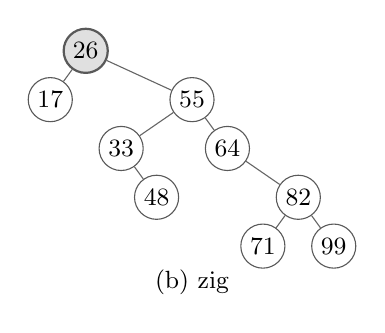
\begin{tikzpicture}[x=0.45cm,y=0.62cm,baseline=(current bounding box.north),tn/.style={circle,draw=black!65,minimum size=0.56cm,inner sep=0pt,font=\small},tnN/.style={thick,fill=black!12},te/.style={draw=black!60},plab/.style={font=\small}]
\node[tn] (ntub17) at (0,-1) {17};
\node[tn,tnN] (ntub26) at (1,0) {26};
\node[tn] (ntub33) at (2,-2) {33};
\node[tn] (ntub48) at (3,-3) {48};
\node[tn] (ntub55) at (4,-1) {55};
\node[tn] (ntub64) at (5,-2) {64};
\node[tn] (ntub71) at (6,-4) {71};
\node[tn] (ntub82) at (7,-3) {82};
\node[tn] (ntub99) at (8,-4) {99};
\draw[te] (ntub26) -- (ntub17);
\draw[te] (ntub26) -- (ntub55);
\draw[te] (ntub55) -- (ntub33);
\draw[te] (ntub33) -- (ntub48);
\draw[te] (ntub55) -- (ntub64);
\draw[te] (ntub64) -- (ntub82);
\draw[te] (ntub82) -- (ntub71);
\draw[te] (ntub82) -- (ntub99);
\node[plab] at (4.0,-4.75) {(b) zig};
\end{tikzpicture}\hspace{0.3cm}\begin{tikzpicture}[x=0.45cm,y=0.62cm,baseline=(current bounding box.north),tn/.style={circle,draw=black!65,minimum size=0.56cm,inner sep=0pt,font=\small},tnN/.style={thick,fill=black!12},te/.style={draw=black!60},plab/.style={font=\small}]
\node[tn] (ntuc17) at (0,0) {17};
\node[tn] (ntuc33) at (1,-2) {33};
\node[tn] (ntuc48) at (2,-3) {48};
\node[tn] (ntuc55) at (3,-1) {55};
\node[tn] (ntuc64) at (4,-2) {64};
\node[tn] (ntuc71) at (5,-4) {71};
\node[tn] (ntuc82) at (6,-3) {82};
\node[tn] (ntuc99) at (7,-4) {99};
\draw[te] (ntuc17) -- (ntuc55);
\draw[te] (ntuc55) -- (ntuc33);
\draw[te] (ntuc33) -- (ntuc48);
\draw[te] (ntuc55) -- (ntuc64);
\draw[te] (ntuc64) -- (ntuc82);
\draw[te] (ntuc82) -- (ntuc71);
\draw[te] (ntuc82) -- (ntuc99);
\node[plab] at (3.5,-4.75) {(c) 刪掉 26，接上 $R$};
\end{tikzpicture}\\*[0.6em]
\begin{tikzpicture}[x=0.45cm,y=0.62cm,baseline=(current bounding box.north),tn/.style={circle,draw=black!65,minimum size=0.56cm,inner sep=0pt,font=\small},tnN/.style={thick,fill=black!12},te/.style={draw=black!60},plab/.style={font=\small}]
\node[tn] (ntud17) at (0,-4) {17};
\node[tn] (ntud26) at (1,-3) {26};
\node[tn] (ntud33) at (2,-2) {33};
\node[tn] (ntud48) at (3,-1) {48};
\node[tn] (ntud55) at (4,0) {55};
\node[tn] (ntud64) at (5,-1) {64};
\node[tn] (ntud71) at (6,-3) {71};
\node[tn,tnN] (ntud75) at (7,-4) {75};
\node[tn] (ntud82) at (8,-2) {82};
\node[tn] (ntud99) at (9,-3) {99};
\draw[te] (ntud55) -- (ntud48);
\draw[te] (ntud48) -- (ntud33);
\draw[te] (ntud33) -- (ntud26);
\draw[te] (ntud26) -- (ntud17);
\draw[te] (ntud55) -- (ntud64);
\draw[te] (ntud64) -- (ntud82);
\draw[te] (ntud82) -- (ntud71);
\draw[te] (ntud71) -- (ntud75);
\draw[te] (ntud82) -- (ntud99);
\node[plab] at (4.5,-6.75) {(d) 75 接成葉節點};
\end{tikzpicture}\hspace{0.3cm}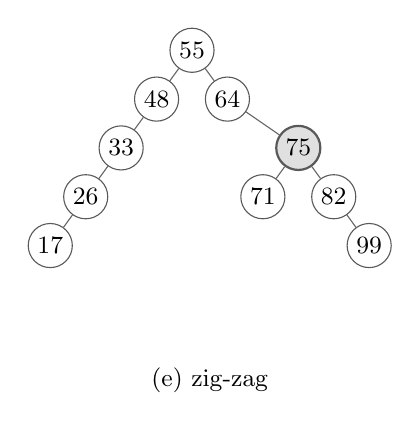
\begin{tikzpicture}[x=0.45cm,y=0.62cm,baseline=(current bounding box.north),tn/.style={circle,draw=black!65,minimum size=0.56cm,inner sep=0pt,font=\small},tnN/.style={thick,fill=black!12},te/.style={draw=black!60},plab/.style={font=\small}]
\node[tn] (ntue17) at (0,-4) {17};
\node[tn] (ntue26) at (1,-3) {26};
\node[tn] (ntue33) at (2,-2) {33};
\node[tn] (ntue48) at (3,-1) {48};
\node[tn] (ntue55) at (4,0) {55};
\node[tn] (ntue64) at (5,-1) {64};
\node[tn] (ntue71) at (6,-3) {71};
\node[tn,tnN] (ntue75) at (7,-2) {75};
\node[tn] (ntue82) at (8,-3) {82};
\node[tn] (ntue99) at (9,-4) {99};
\draw[te] (ntue55) -- (ntue48);
\draw[te] (ntue48) -- (ntue33);
\draw[te] (ntue33) -- (ntue26);
\draw[te] (ntue26) -- (ntue17);
\draw[te] (ntue55) -- (ntue64);
\draw[te] (ntue64) -- (ntue75);
\draw[te] (ntue75) -- (ntue71);
\draw[te] (ntue75) -- (ntue82);
\draw[te] (ntue82) -- (ntue99);
\node[plab] at (4.5,-6.75) {(e) zig-zag};
\end{tikzpicture}\hspace{0.3cm}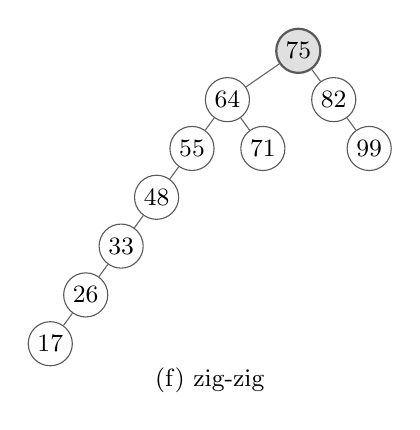
\begin{tikzpicture}[x=0.45cm,y=0.62cm,baseline=(current bounding box.north),tn/.style={circle,draw=black!65,minimum size=0.56cm,inner sep=0pt,font=\small},tnN/.style={thick,fill=black!12},te/.style={draw=black!60},plab/.style={font=\small}]
\node[tn] (ntuf17) at (0,-6) {17};
\node[tn] (ntuf26) at (1,-5) {26};
\node[tn] (ntuf33) at (2,-4) {33};
\node[tn] (ntuf48) at (3,-3) {48};
\node[tn] (ntuf55) at (4,-2) {55};
\node[tn] (ntuf64) at (5,-1) {64};
\node[tn] (ntuf71) at (6,-2) {71};
\node[tn,tnN] (ntuf75) at (7,0) {75};
\node[tn] (ntuf82) at (8,-1) {82};
\node[tn] (ntuf99) at (9,-2) {99};
\draw[te] (ntuf75) -- (ntuf64);
\draw[te] (ntuf64) -- (ntuf55);
\draw[te] (ntuf55) -- (ntuf48);
\draw[te] (ntuf48) -- (ntuf33);
\draw[te] (ntuf33) -- (ntuf26);
\draw[te] (ntuf26) -- (ntuf17);
\draw[te] (ntuf64) -- (ntuf71);
\draw[te] (ntuf75) -- (ntuf82);
\draw[te] (ntuf82) -- (ntuf99);
\node[plab] at (4.5,-6.75) {(f) zig-zig};
\end{tikzpicture}
\end{center}
\begin{itemize}
\item[(A)] 錯。 (c) 裡 $33$ 的父節點是 $55$；$48$ 反而是 $33$ 的子節點。
\item[(B)] 對。 (c) 的根是 $17$。
\item[(C)] 錯。 (f) 裡 $99$ 在根 $75$ 的右子樹（$82$ 底下），$64$ 在左子樹，不是 $99$ 的祖先。
\item[(D)] 對。 (f) 裡 $55 \to 48 \to 33$，$33$ 是 $55$ 的子孫。
\item[(E)] 對。 插入後伸展新節點，$75$ 一定在根。
\end{itemize}
\end{pastsoln}
